%=============================================================================
% Chapter 3: One-Dimensional Arrays
%=============================================================================
\chapter{One-Dimensional Arrays}
\label{ch:one-dimensional-arrays}

%-----------------------------------------------------------------------------
\section{Introduction to Arrays}
\label{sec:intro-arrays}
%-----------------------------------------------------------------------------

In many programming situations, we need to store and manipulate collections of
related data items---for instance, the grades of all students in a class or the
daily temperatures over a month. Declaring a separate variable for each value
quickly becomes impractical. \emph{Arrays} provide an elegant solution.

\begin{definitionbox}{Array}
An \textbf{array} is a consecutive group of homogeneous memory locations that
all share the same name and the same data type. Each individual location is
called an \textbf{element} and is accessed through an \textbf{index}
(subscript).
\end{definitionbox}

Key characteristics of arrays:
\begin{itemize}
    \item All elements occupy \emph{contiguous} (adjacent) memory locations.
    \item Every element is of the \emph{same} data type.
    \item Elements are referenced by combining the array name with a
          non-negative integer index enclosed in square brackets.
    \item Arrays can hold simple built-in types (\texttt{int}, \texttt{float},
          \texttt{double}, \texttt{char}) as well as user-defined types.
\end{itemize}

\begin{infobox}{Why Use Arrays?}
Without arrays, storing ten exam scores would require ten separate variables
(\texttt{score0}, \texttt{score1}, \ldots, \texttt{score9}). With an array we
write \texttt{int score[10];} and access each value through its index---much
cleaner, and far easier to process with loops.
\end{infobox}

%-----------------------------------------------------------------------------
\section{Declaring One-Dimensional Arrays}
\label{sec:declaring-arrays}
%-----------------------------------------------------------------------------

A one-dimensional array is the simplest form of an array. Its declaration
follows the general syntax:

\begin{conceptbox}{Array Declaration Syntax}
\begin{verbatim}
    data-type  Array-name[size];
\end{verbatim}
\begin{itemize}
    \item \texttt{data-type} --- the type of each element
          (e.g.\ \texttt{int}, \texttt{float}, \texttt{char}).
    \item \texttt{Array-name} --- a valid C++ identifier.
    \item \texttt{size} --- a positive integer constant specifying
          the number of elements.
\end{itemize}
\end{conceptbox}

\paragraph{Examples.}

\begin{cppcode}
int   age[10];    // 10 integers
int   num[30];    // 30 integers
float degree[5];  // 5 floating-point numbers
char  a[15];      // 15 characters
\end{cppcode}

\begin{warningbox}{Array Size Must Be a Constant}
In standard C++, the size of an array must be a compile-time constant
expression. Using a variable as the size (variable-length arrays) is not
part of the C++ standard, although some compilers accept it as an extension.
\end{warningbox}

\subsection*{Visualising an Array in Memory}

The following diagram illustrates an integer array \texttt{age} of size~10.
Each box represents one element; the numbers above the boxes are the indices
(0 through~9).

\begin{center}
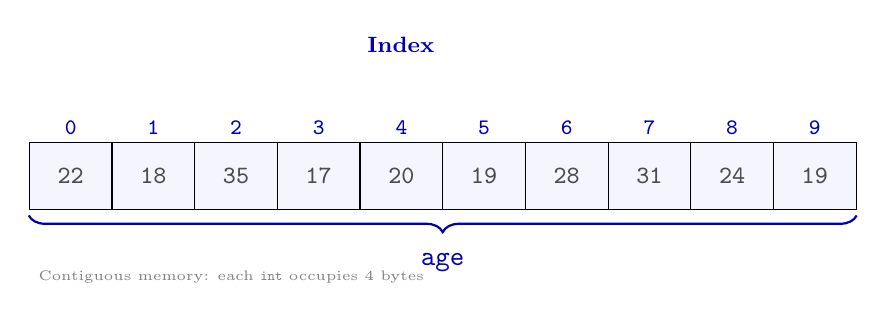
\begin{tikzpicture}[
    cell/.style={
        draw,
        minimum width=1.05cm,
        minimum height=0.85cm,
        anchor=south west,
        font=\small,
        fill=blue!4
    },
    idx/.style={
        font=\footnotesize\ttfamily\bfseries,
        text=blue!70!black
    },
    val/.style={
        font=\small\ttfamily,
        text=black!70
    }
]
% Index heading
\node[font=\footnotesize\bfseries, text=blue!70!black]
    at (4.725, 2.1) {Index};

% Draw cells with index numbers and sample values
\foreach \i/\v in {0/22,1/18,2/35,3/17,4/20,5/19,6/28,7/31,8/24,9/19} {
    \node[cell] (c\i) at (\i*1.05, 0) {};
    % Index on top
    \node[idx] at ([yshift=5pt]c\i.north) {\i};
    % Sample value inside
    \node[val] at (c\i.center) {\v};
}

% Array name brace below
\draw[decorate,
      decoration={brace, amplitude=6pt, mirror},
      thick, blue!70!black]
    ([yshift=-2pt]c0.south west) -- ([yshift=-2pt]c9.south east)
    node[midway, below=10pt, font=\bfseries\ttfamily,
         text=blue!70!black] {age};

% Address hint
\node[font=\tiny, text=gray, anchor=west] at (0, -0.85)
    {Contiguous memory: each \texttt{int} occupies 4 bytes};
\end{tikzpicture}
\end{center}

\begin{infobox}{Memory Layout Detail}
When you declare \texttt{int age[10];}, the compiler allocates
$10 \times \texttt{sizeof(int)} = 10 \times 4 = 40$~bytes of contiguous
memory. The address of element \texttt{age[i]} is
\texttt{base\_address + i\,*\,sizeof(int)}.
This is why array access by index is an $O(1)$ operation.
\end{infobox}

%-----------------------------------------------------------------------------
\section{Initialising Array Elements}
\label{sec:initialising-arrays}
%-----------------------------------------------------------------------------

There are several ways to assign initial values to the elements of an array.

\subsection{Individual Element Initialisation}

Each element can be assigned a value independently:

\begin{cppcode}
age[0] = 18;
age[9] = 19;
\end{cppcode}

\subsection{Initialiser-List Initialisation}

All elements can be initialised at the point of declaration using an
\emph{initialiser list}:

\begin{cppcode}
int age[9] = {18, 17, 18, 18, 19, 20, 17, 18, 19};
\end{cppcode}

\subsection{Auto-Sized Initialisation}

When an initialiser list is provided, the compiler can deduce the size of the
array automatically:

\begin{cppcode}
int x[] = {12, 3, 5, 0, 11, 7, 30, 100, 22};  // size = 9
\end{cppcode}

\subsection{Partial Initialisation with Explicit Size}

If fewer initialisers are provided than the declared size, the remaining
elements are automatically initialised to zero:

\begin{cppcode}
int y[10] = {8, 10, 13, 15, 0, 1, 17, 22};
// y[8] and y[9] are automatically set to 0
\end{cppcode}

\begin{importantbox}{Zero-Initialisation Shortcut}
To set every element of an array to zero, write:
\begin{verbatim}
    int arr[100] = {0};
\end{verbatim}
The first element is explicitly set to \texttt{0}, and the rest are
zero-initialised by the partial-initialisation rule.
\end{importantbox}

The following table summarises all four initialisation methods:

\begin{center}
\renewcommand{\arraystretch}{1.4}
\begin{tabular}{@{} l l @{}}
\toprule
\textbf{Method} & \textbf{Syntax Example} \\
\midrule
Individual assignment & \texttt{age[0] = 18; age[1] = 17;} \\
Full initialiser list & \texttt{int a[3] = \{10, 20, 30\};} \\
Auto-sized            & \texttt{int a[] = \{10, 20, 30\};} \\
Partial (rest = 0)    & \texttt{int a[5] = \{10, 20\};} \\
\bottomrule
\end{tabular}
\end{center}

%-----------------------------------------------------------------------------
\section{Accessing Array Elements}
\label{sec:accessing-arrays}
%-----------------------------------------------------------------------------

Individual elements are accessed by appending the index in square brackets to
the array name. The index of the \emph{first} element is always~\texttt{0};
the index of the \emph{last} element is \texttt{size\,-\,1}.

\begin{cppcode}
int x, y;
x = num[0];   // copy the first element into x
y = num[9];   // copy the tenth element into y
\end{cppcode}

Array elements can participate in any expression, just like ordinary
variables:

\begin{cppcode}
cout << num[0] + num[9];     // print the sum
num[0] = num[1] + num[2];   // assign the sum
num[7] += 3;                 // increment by 3
\end{cppcode}

\begin{warningbox}{Index Out of Bounds}
C++ does \textbf{not} perform automatic bounds checking on array indices. If
you access \texttt{num[10]} in a 10-element array (valid indices 0--9), the
behaviour is \emph{undefined}---your program may crash, produce garbage
values, or corrupt other data.
\end{warningbox}

%-----------------------------------------------------------------------------
\section{Reading, Writing, and Processing Arrays}
\label{sec:rwp-arrays}
%-----------------------------------------------------------------------------

Because arrays work hand-in-hand with loops, nearly all array processing uses
a \texttt{for} loop whose counter variable serves as the index.

\subsection{Writing (Printing) a Single Element}

\begin{cppcode}
cout << num[4];   // print the element at index 4
\end{cppcode}

\subsection{Reading an Array from the User}

\begin{cppcode}
#include <iostream>
using namespace std;

int main() {
    int num[10];

    cout << "Enter 10 integers:" << endl;
    for (int i = 0; i < 10; i++) {
        cin >> num[i];
    }

    return 0;
}
\end{cppcode}

\subsection{Printing an Array in Forward Order}

\begin{cppcode}
cout << "Array elements (forward):" << endl;
for (int i = 0; i < 10; i++) {
    cout << num[i] << " ";
}
cout << endl;
\end{cppcode}

\subsection{Printing an Array in Reverse Order}

\begin{cppcode}
cout << "Array elements (reverse):" << endl;
for (int i = 9; i >= 0; i--) {
    cout << num[i] << " ";
}
cout << endl;
\end{cppcode}

\subsection{Computing the Sum of All Elements}

\begin{cppcode}
int sum = 0;
for (int i = 0; i < 10; i++) {
    sum += num[i];
}
cout << "Sum = " << sum << endl;
\end{cppcode}

%-----------------------------------------------------------------------------
\section{Practical Examples}
\label{sec:array-examples}
%-----------------------------------------------------------------------------

\subsection{Example 1: Accessing Specific Elements}

\textbf{Problem.} Given the array
\texttt{double distance[] = \{23.14, 70.52, 104.08, 468.78, 6.28\}},
display the 2nd and 5th elements.

\begin{cppcode}
#include <iostream>
using namespace std;

int main() {
    double distance[] = {23.14, 70.52, 104.08,
                         468.78, 6.28};

    cout << "2nd element: " << distance[1] << endl;
    cout << "5th element: " << distance[4] << endl;

    return 0;
}
\end{cppcode}

\textbf{Output:}
\begin{verbatim}
2nd element: 70.52
5th element: 6.28
\end{verbatim}

\begin{infobox}{Indexing Starts at Zero}
The ``2nd element'' is at index~1, and the ``5th element'' is at index~4.
Always remember: the $k$-th element is at index $k - 1$.
\end{infobox}

%--------------------------------------------------------------------
\subsection{Example 2: Read and Print in Reverse}

\textbf{Problem.} Read 5 numbers from the user and print them in reverse
order.

\begin{cppcode}
#include <iostream>
using namespace std;

int main() {
    int arr[5];

    cout << "Enter 5 numbers:" << endl;
    for (int i = 0; i < 5; i++) {
        cin >> arr[i];
    }

    cout << "Numbers in reverse order:" << endl;
    for (int i = 4; i >= 0; i--) {
        cout << arr[i] << " ";
    }
    cout << endl;

    return 0;
}
\end{cppcode}

\textbf{Sample run:}
\begin{verbatim}
Enter 5 numbers:
10 20 30 40 50
Numbers in reverse order:
50 40 30 20 10
\end{verbatim}

%--------------------------------------------------------------------
\subsection{Example 3: Summation of Array Elements}

\textbf{Problem.} Read 10 integers into an array and compute their
summation.

\begin{cppcode}
#include <iostream>
using namespace std;

int main() {
    int arr[10];
    int sum = 0;

    cout << "Enter 10 integers:" << endl;
    for (int i = 0; i < 10; i++) {
        cin >> arr[i];
    }

    for (int i = 0; i < 10; i++) {
        sum += arr[i];
    }

    cout << "Summation = " << sum << endl;

    return 0;
}
\end{cppcode}

\textbf{Sample run:}
\begin{verbatim}
Enter 10 integers:
1 2 3 4 5 6 7 8 9 10
Summation = 55
\end{verbatim}

%--------------------------------------------------------------------
\subsection{Example 4: Finding the Minimum Value}

\textbf{Problem.} Read 8 numbers into an array and find the minimum
value.

\begin{cppcode}
#include <iostream>
using namespace std;

int main() {
    int arr[8];

    cout << "Enter 8 numbers:" << endl;
    for (int i = 0; i < 8; i++) {
        cin >> arr[i];
    }

    int min = arr[0];
    for (int i = 1; i < 8; i++) {
        if (arr[i] < min) {
            min = arr[i];
        }
    }

    cout << "Minimum value = " << min << endl;

    return 0;
}
\end{cppcode}

\textbf{Sample run:}
\begin{verbatim}
Enter 8 numbers:
34 12 56 7 89 23 45 11
Minimum value = 7
\end{verbatim}

\begin{infobox}{Finding the Minimum --- Strategy}
\begin{enumerate}
    \item Assume the first element is the minimum.
    \item Compare it with every subsequent element.
    \item Whenever a smaller element is found, update the minimum.
    \item After the loop completes, the variable holds the true
          minimum.
\end{enumerate}
\end{infobox}

%--------------------------------------------------------------------
\subsection{Example 5: Days in Each Month}

\textbf{Problem.} Use an array to store the number of days in each
month (non-leap year) and display them.

\begin{cppcode}
#include <iostream>
using namespace std;

int main() {
    int days[] = {31, 28, 31, 30, 31, 30,
                  31, 31, 30, 31, 30, 31};

    string months[] = {
        "January",   "February", "March",
        "April",     "May",      "June",
        "July",      "August",   "September",
        "October",   "November", "December"
    };

    for (int i = 0; i < 12; i++) {
        cout << months[i] << " has "
             << days[i] << " days." << endl;
    }

    return 0;
}
\end{cppcode}

\textbf{Output (first four lines shown):}
\begin{verbatim}
January has 31 days.
February has 28 days.
March has 31 days.
April has 30 days.
...
\end{verbatim}

\begin{conceptbox}{Parallel Arrays}
Using two arrays of the same size---one for month names and one for day
counts---is called the \textbf{parallel array} technique. The element at
index~\texttt{i} in one array corresponds to the element at the same
index in the other.
\end{conceptbox}

%--------------------------------------------------------------------
\subsection{Example 6: Searching for a Value (Using a Function)}

\textbf{Problem.} Write a function that searches for a value \texttt{X}
in an array and returns its index. If the value is not found,
return~\texttt{-1}.

\begin{cppcode}
#include <iostream>
using namespace std;

int search(int arr[], int size, int x) {
    for (int i = 0; i < size; i++) {
        if (arr[i] == x) {
            return i;   // found: return the index
        }
    }
    return -1;          // not found
}

int main() {
    int arr[] = {10, 25, 33, 47, 52, 68, 71, 89};
    int size = 8;
    int x;

    cout << "Enter a value to search for: ";
    cin >> x;

    int index = search(arr, size, x);

    if (index != -1) {
        cout << x << " found at index "
             << index << endl;
    } else {
        cout << x << " not found in the array."
             << endl;
    }

    return 0;
}
\end{cppcode}

\textbf{Sample run 1:}
\begin{verbatim}
Enter a value to search for: 47
47 found at index 3
\end{verbatim}

\textbf{Sample run 2:}
\begin{verbatim}
Enter a value to search for: 99
99 not found in the array.
\end{verbatim}

\begin{conceptbox}{Linear Search}
The algorithm shown above is called \textbf{linear search} (or
\emph{sequential search}). It examines each element one by one from the
beginning of the array until the target value is found or the end of the
array is reached. Its time complexity is $O(n)$.
\end{conceptbox}

%--------------------------------------------------------------------
\subsection{Example 7: Splitting Odd and Even Numbers}

\textbf{Problem.} Read 10 integers into an array, then split them into
two separate arrays: one for odd numbers and one for even numbers.

\begin{cppcode}
#include <iostream>
using namespace std;

int main() {
    int arr[10];
    int odd[10], even[10];
    int oddCount = 0, evenCount = 0;

    cout << "Enter 10 integers:" << endl;
    for (int i = 0; i < 10; i++) {
        cin >> arr[i];
    }

    for (int i = 0; i < 10; i++) {
        if (arr[i] % 2 == 0) {
            even[evenCount] = arr[i];
            evenCount++;
        } else {
            odd[oddCount] = arr[i];
            oddCount++;
        }
    }

    cout << "Even numbers: ";
    for (int i = 0; i < evenCount; i++) {
        cout << even[i] << " ";
    }
    cout << endl;

    cout << "Odd numbers: ";
    for (int i = 0; i < oddCount; i++) {
        cout << odd[i] << " ";
    }
    cout << endl;

    return 0;
}
\end{cppcode}

\textbf{Sample run:}
\begin{verbatim}
Enter 10 integers:
3 8 15 22 7 40 11 6 9 18
Even numbers: 8 22 40 6 18
Odd numbers: 3 15 7 11 9
\end{verbatim}

\begin{importantbox}{Tracking Array Sizes with Counters}
When the number of elements to be stored in an array is not known in
advance, maintain a separate counter variable (e.g.\ \texttt{oddCount},
\texttt{evenCount}) that tracks how many elements have been inserted so
far. This counter also serves as the index for the next insertion.
\end{importantbox}
